\documentclass{standalone}

% Font
\usepackage{mathpazo}
\usepackage{libertine}
\renewcommand*\sfdefault{phv}

\large

% Color
\usepackage{xcolor}
\definecolor{f1}{HTML}{F39019}
\definecolor{b1}{HTML}{DE6A10}
\definecolor{f2}{HTML}{51A7F9}
\definecolor{b2}{HTML}{0365C0}
\definecolor{f3}{HTML}{70BF41}
\definecolor{b3}{HTML}{00882B}

% tikz
\usepackage{tikz}
\tikzstyle{every node}=[font=\sffamily]
\usetikzlibrary{shapes,arrows,positioning,calc,decorations.markings,backgrounds}
\tikzstyle{c1} = [thick,draw=b1,fill=f1]
\tikzstyle{c2} = [thick,draw=b2,fill=f2]
\tikzstyle{c3} = [thick,draw=b3,fill=f3]
\tikzstyle{cg} = [thick,draw=gray!50,fill=gray!30]
\tikzstyle{rect} = [rectangle, minimum height=1cm]
\tikzstyle{roundrect} = [rect, rounded corners=.2cm]
\tikzstyle{io} = [trapezium, trapezium left angle=70, trapezium right angle=110]
\tikzstyle{arrow} = [thick,->,>=stealth]

\tikzstyle{des}=[a1, align=center]
\tikzstyle{ma}=[-stealth, line width=1pt, a1]

\begin{document}
	
\begin{tikzpicture}

\begin{scope}
	\node[anchor=south west,inner sep=0] (image) at (0,0) {
		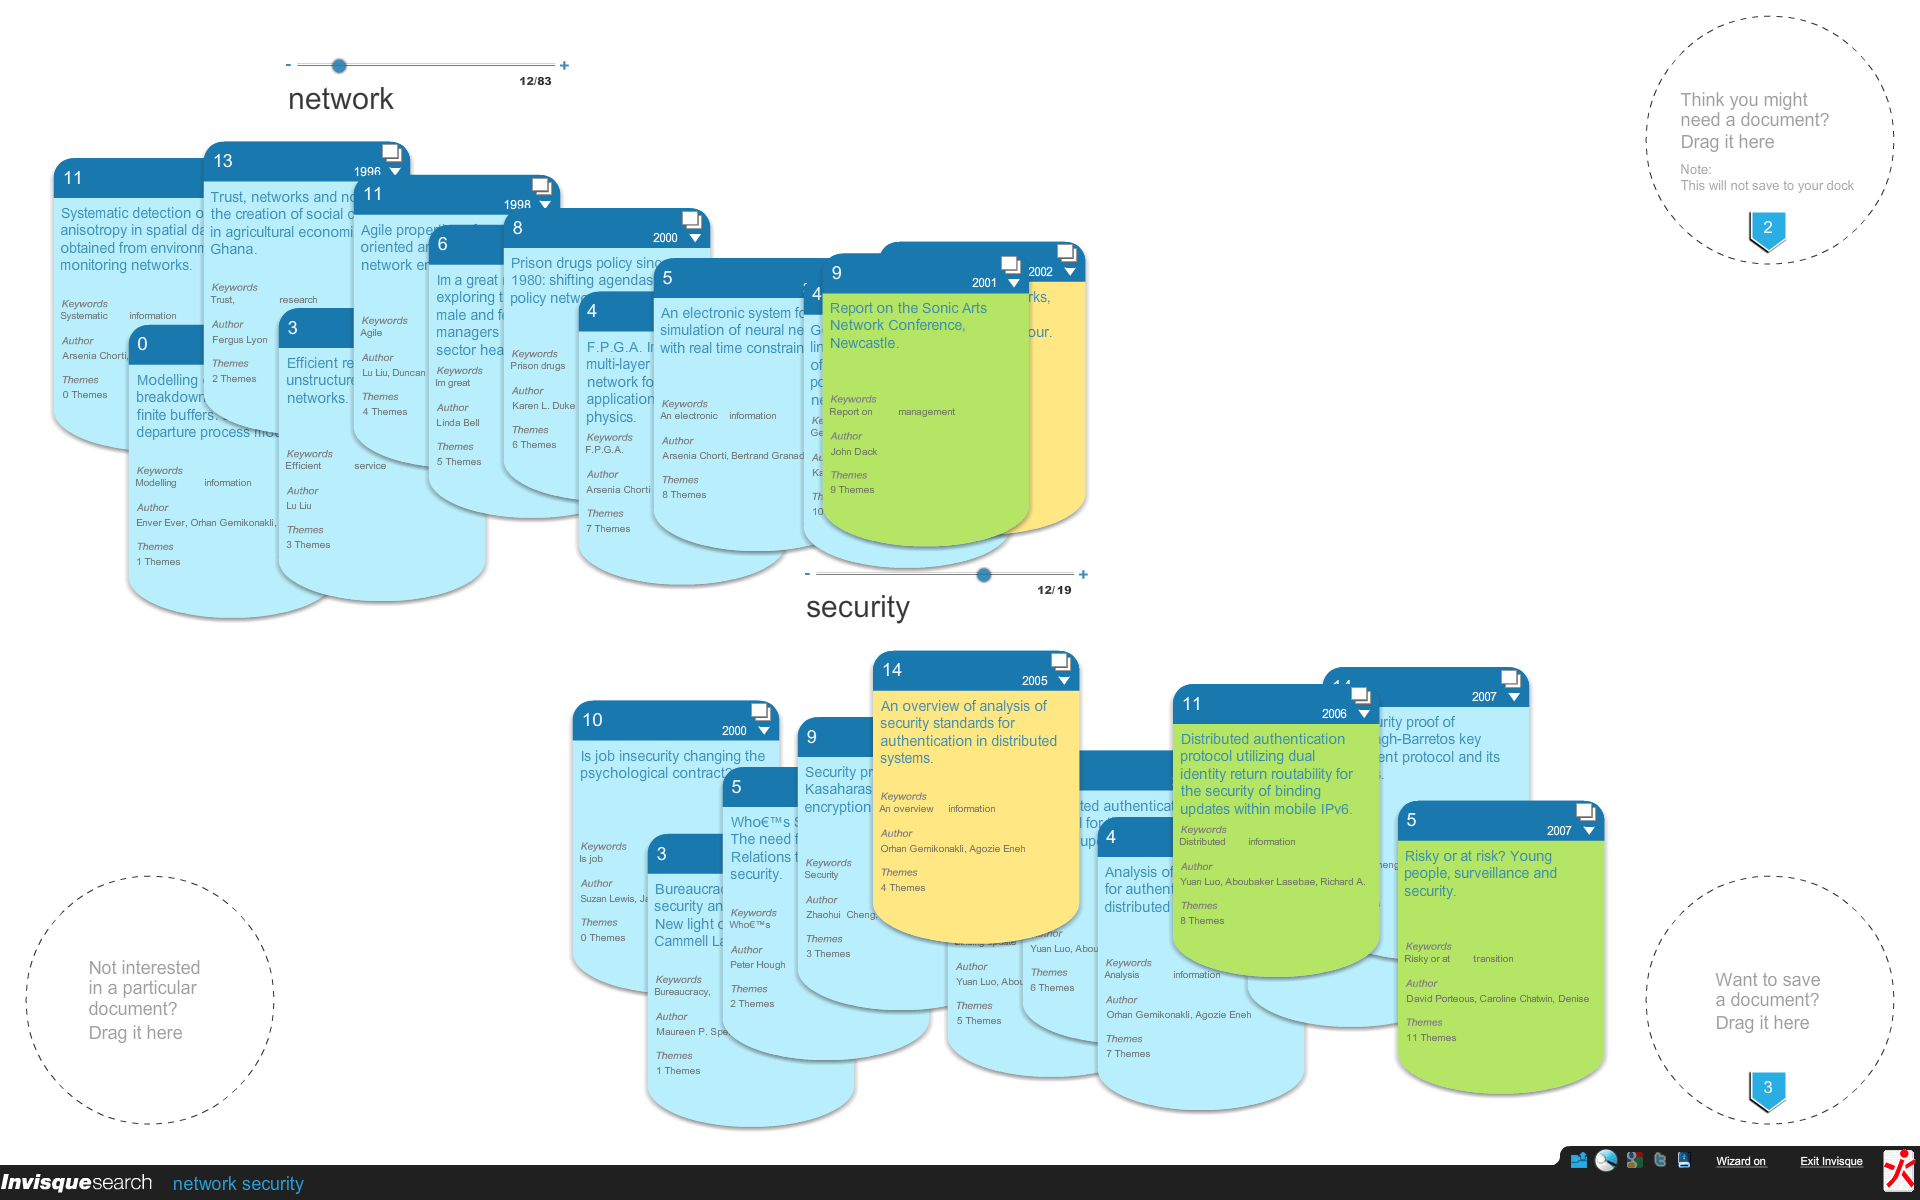
\includegraphics[width=\linewidth]{invisque-raw}
	};
		
	\begin{scope}[x={(image.south east)},y={(image.north west)}]
		\node [des] (citation) at (.4,.95) { citation \\count };
		\node [des] (year) at (.6,.95) { publication \\year };
		\node [des, anchor=west] (title) at (.58,.73) { title };
		\node [des, anchor=west] (keywords) at (.58,.65) { keywords };
		\node [des, anchor=west] (author) at (.55,.55) { authors };
		\draw [ma] (citation) -- ++(.03,-.16);
		\draw [ma] (year) -- ++(-.08,-.16);
		\draw [ma] (title) -- ++(-.11,0);
		\draw [ma] (keywords) -- ++(-.16,0);
		\draw [ma] (author) -- ++(-.16,.07);
	\end{scope}
\end{scope}

\end{tikzpicture}

\end{document}